\chapter{Ripasso: dal Machine Learning alle reti neurali}\label{ch:ripasso}
Il Deep Learning non nasce dal nulla: le reti neurali profonde riutilizzano quasi tutti gli strumenti già visti nel Machine Learning classico, ovvero un modello parametrico, una funzione di loss da minimizzare, la discesa del gradiente e la regolarizzazione. In questo capitolo riprendiamo questi strumenti partendo dalla regressione logistica e dal modello softmax, mostriamo che il softmax può già essere visto come una rete neurale molto semplice e arriviamo, attraverso il problema della rappresentazione dei dati, al Multi-Layer Perceptron. Il capitolo si chiude con la domanda che motiva tutto il capitolo successivo: come si calcolano i gradienti di una rete con uno o più hidden layer?

\section{Gli ingredienti di un algoritmo di Machine Learning}
Qualunque algoritmo di Machine Learning supervisionato che vedremo è costruito a partire dagli stessi elementi:
\begin{itemize}
    \item \textbf{Un modello}: una funzione $h_\vartheta$ che, dato un input $x$, restituisce una predizione.
    \item \textbf{Dei parametri}: il vettore (o la matrice) $\vartheta$ che determina il comportamento del modello e che va appreso dai dati.
    \item \textbf{Un set di dati}: il training set $\mathcal{D} = \{(x^{(1)}, y^{(1)}), \dots, (x^{(m)}, y^{(m)})\}$, composto da $m$ esempi etichettati.
    \item \textbf{Un algoritmo di learning}: la procedura che, minimizzando una funzione di costo $J(\vartheta)$, trova i parametri migliori per il modello.
\end{itemize}

Ogni input $x^{(i)}$ è un vettore di $n$ feature. Per semplificare la notazione si aggiunge in testa una feature fittizia $x_0^{(i)} = 1$, detta \textbf{bias}, in modo che il termine noto del modello possa essere trattato come un parametro qualunque:
\[
x^{(i)} = \begin{bmatrix} x_0^{(i)} \\ x_1^{(i)} \\ \vdots \\ x_n^{(i)} \end{bmatrix} \in \mathbb{R}^{n+1}, \qquad x_0^{(i)} = 1
\]
dove $x_1^{(i)}, \dots, x_n^{(i)}$ sono le feature vere e proprie dell'$i$-esimo esempio.

\paragraph{Discesa del gradiente.}
Come algoritmo di learning useremo quasi sempre la \textbf{discesa del gradiente}, ovvero un metodo iterativo che aggiorna i parametri nella direzione opposta al gradiente della funzione di costo:
\[
\vartheta_j \leftarrow \vartheta_j - \alpha \frac{\partial J(\vartheta)}{\partial \vartheta_j} \qquad \forall j \text{ simultaneamente}
\]
dove $\alpha > 0$ è il \textbf{learning rate}, un iperparametro che controlla l'ampiezza del passo. Valori tipici si scelgono su una scala approssimativamente logaritmica, ad esempio $0.1,\ 0.03,\ 0.01,\ 0.003,\ 0.001$: un $\alpha$ troppo grande rischia di far divergere l'algoritmo, mentre uno troppo piccolo rende la convergenza molto lenta.

\paragraph{Regolarizzazione.}
L'overfitting è uno dei problemi che si possono incontrare durante il training di un modello. Per contrastarlo si aggiunge alla funzione di costo un \textbf{termine di regolarizzazione}, che penalizza parametri di valore elevato:
\[
J(\vartheta) = \underbrace{-\frac{1}{m}\Big[\cdots\Big]}_{\text{loss sui dati}} + \underbrace{\frac{\lambda}{2m}\sum_{j=1}^{n}\vartheta_j^2}_{\text{regolarizzazione}}
\]
dove $\lambda$ controlla l'intensità della penalizzazione e, tipicamente, il parametro del bias $\vartheta_0$ non viene regolarizzato. Un $\lambda$ grande porta a modelli più semplici, ma se è troppo grande il modello rischia di andare in underfitting.

\section{Regressione logistica}
La \textbf{regressione logistica} è il framework di learning per distinguere tra due classi, ovvero per la classificazione binaria con $y^{(i)} \in \{0, 1\}$. Il modello applica la funzione \textbf{sigmoide} a una combinazione lineare delle feature:
\[
h_\vartheta(x) = \sigma(\vartheta^T x) = \frac{1}{1 + e^{-\vartheta^T x}}, \qquad \vartheta = [\vartheta_0, \vartheta_1, \dots, \vartheta_n]^T \in \mathbb{R}^{n+1}
\]
e restituisce quindi un valore in $(0, 1)$, interpretabile come la probabilità $P(y = 1 \mid x)$.

La funzione di costo è la \textbf{cross-entropy loss} (o binary cross-entropy):
\[
J(\vartheta) = -\frac{1}{m}\sum_{i=1}^{m}\Big[y^{(i)}\log h_\vartheta(x^{(i)}) + (1 - y^{(i)})\log\big(1 - h_\vartheta(x^{(i)})\big)\Big]
\]
che penalizza fortemente le predizioni sicure ma sbagliate: se $y^{(i)} = 1$ e $h_\vartheta(x^{(i)}) \to 0$ (o viceversa) la loss diverge. I parametri si trovano con la discesa del gradiente e, se necessario, con la regolarizzazione vista sopra.

Per eseguire una classificazione multiclasse con la regressione logistica si può ricorrere all'approccio \textbf{one vs all}, addestrando un classificatore binario per ogni classe. Questa strategia presenta però diverse criticità: il numero di classificatori cresce con il numero di classi, possono comparire regioni di incertezza e le probabilità restituite dai singoli classificatori non sono facilmente confrontabili. Per questo motivo si introduce un modello pensato direttamente per il caso multiclasse.

\section{Softmax}\label{sec:softmax}
Il \textbf{softmax} è il framework di learning per eseguire la classificazione multiclasse, ed è un'estensione della regressione logistica. Le etichette appartengono ora a $K$ classi, $y^{(i)} \in \{0, 1, \dots, K-1\}$, e vengono rappresentate con il \textbf{one-hot encoding}, ovvero come un vettore di $K$ componenti tutte nulle tranne quella corrispondente alla classe corretta, che vale 1.

\subsection{Il modello}
Dato un input $x$, vogliamo stimare la probabilità che appartenga a ciascuna delle classi:
\[
P_\vartheta(y = k \mid x) \qquad \forall k = 0, 1, \dots, K-1.
\]
La nostra ipotesi deve quindi stimare un vettore di $K$ probabilità, e per farlo ogni classe $k$ ha il proprio vettore di parametri $\vartheta^{(k)} \in \mathbb{R}^{n+1}$.

\begin{definizione}[Modello softmax]
Il modello softmax restituisce la distribuzione di probabilità sulle $K$ classi:
\[
h_\vartheta(x) =
\begin{bmatrix}
P_\vartheta(y = 0 \mid x) \\ P_\vartheta(y = 1 \mid x) \\ \vdots \\ P_\vartheta(y = K-1 \mid x)
\end{bmatrix}
= \frac{1}{\displaystyle\sum_{k=0}^{K-1} e^{\vartheta^{(k)T} x}}
\begin{bmatrix}
e^{\vartheta^{(0)T} x} \\ e^{\vartheta^{(1)T} x} \\ \vdots \\ e^{\vartheta^{(K-1)T} x}
\end{bmatrix}
\]
ovvero, per la singola classe $c$:
\[
h_\vartheta^{(c)}(x) = P_\vartheta(y = c \mid x) = \frac{e^{\vartheta^{(c)T} x}}{\displaystyle\sum_{k=0}^{K-1} e^{\vartheta^{(k)T} x}}.
\]
\end{definizione}

Il denominatore normalizza la distribuzione, per cui, una volta fissati (appresi) i parametri, la somma delle probabilità restituite è sempre pari a 1:
\[
\sum_{k=0}^{K-1} P_\vartheta(y = k \mid x) = 1.
\]
I parametri del modello non sono più un vettore ma una matrice, in cui la colonna $k$-esima contiene i parametri $\vartheta^{(k)}$ della classe $k$:
\[
\vartheta =
\begin{bmatrix}
\vartheta_0^{(0)} & \vartheta_0^{(1)} & \cdots & \vartheta_0^{(K-1)} \\
\vartheta_1^{(0)} & \vartheta_1^{(1)} & \cdots & \vartheta_1^{(K-1)} \\
\vdots & \vdots & \ddots & \vdots \\
\vartheta_n^{(0)} & \vartheta_n^{(1)} & \cdots & \vartheta_n^{(K-1)}
\end{bmatrix}
\in \mathbb{R}^{(n+1) \times K}.
\]

\subsection{Funzione di costo e learning}
Anche il softmax usa la cross-entropy loss, che confronta il vettore one-hot dell'etichetta con le probabilità uscite dal modello. Per scriverla definiamo la \textbf{funzione indicatrice}:
\[
\mathbf{1}\{\text{proposizione}\} =
\begin{cases}
1 & \text{se la proposizione è vera} \\
0 & \text{se la proposizione è falsa}
\end{cases}
\]
La funzione di costo del softmax è quindi:
\[
J(\vartheta) = -\frac{1}{m}\left[\sum_{i=1}^{m}\sum_{c=0}^{K-1}\mathbf{1}\{y^{(i)} = c\}\log h_\vartheta^{(c)}(x^{(i)})\right] + \underbrace{\frac{\lambda}{2m}\sum_{c=0}^{K-1}\sum_{j=1}^{n}\big(\vartheta_j^{(c)}\big)^2}_{\text{regolarizzazione}}
\]
dove, per ogni esempio, sopravvive solo il termine della classe corretta: la loss è quindi $-\log$ della probabilità assegnata alla classe giusta.

L'obiettivo del learning è trovare i parametri che minimizzano $J(\vartheta)$, cosa che si fa con la discesa del gradiente (o con la sua versione stocastica). La derivata parziale rispetto al generico parametro vale:
\[
\frac{\partial J(\vartheta)}{\partial \vartheta_j^{(c)}} = -\frac{1}{m}\sum_{i=1}^{m}\Big[\big(\mathbf{1}\{y^{(i)} = c\} - h_\vartheta^{(c)}(x^{(i)})\big)\,x_j^{(i)}\Big] + \frac{\lambda}{m}\vartheta_j^{(c)}
\]
e l'aggiornamento viene ripetuto fino a convergenza:
\[
\vartheta_j^{(c)} \leftarrow \vartheta_j^{(c)} - \alpha\frac{\partial J(\vartheta)}{\partial \vartheta_j^{(c)}} \qquad \forall j = 0, \dots, n,\ \forall c = 0, \dots, K-1 \text{ simultaneamente.}
\]

\begin{osservazione}[Gradiente rispetto ai logit]
Chiamiamo \textbf{logit} le quantità $z_k = \vartheta^{(k)T}x$, ovvero i valori prima della normalizzazione. Per un singolo esempio, il gradiente della cross-entropy rispetto a ciascun logit ha una forma molto semplice:
\[
\delta_k = \frac{\partial L}{\partial z_k} = p_k - y_k
\]
dove $p_k$ è la probabilità predetta e $y_k$ la componente $k$-esima del vettore one-hot. Il gradiente rispetto al peso che collega la feature $x_j$ al nodo $k$ è poi semplicemente $\delta_k x_j$, mentre quello rispetto al bias è $\delta_k$. È la stessa espressione della formula precedente, letta nodo per nodo: questa idea di \emph{errore locale} propagato all'indietro tornerà nel capitolo~\ref{ch:backprop}.
\end{osservazione}

\subsection{Overparametrizzazione}
Il modello softmax è \textbf{overparametrizzato}, ovvero, per ogni ipotesi che descrive i dati, esistono infinite configurazioni dei parametri che producono esattamente la stessa mappa dagli input $x$ alle predizioni. Infatti, sottraendo a ogni vettore $\vartheta^{(k)}$ lo stesso vettore arbitrario $\psi \in \mathbb{R}^{n+1}$:
\[
\frac{e^{(\vartheta^{(c)} - \psi)^T x}}{\displaystyle\sum_{k=0}^{K-1} e^{(\vartheta^{(k)} - \psi)^T x}}
= \frac{e^{\vartheta^{(c)T} x}\, e^{-\psi^T x}}{e^{-\psi^T x}\displaystyle\sum_{k=0}^{K-1} e^{\vartheta^{(k)T} x}}
= \frac{e^{\vartheta^{(c)T} x}}{\displaystyle\sum_{k=0}^{K-1} e^{\vartheta^{(k)T} x}}
\]
il fattore comune $e^{-\psi^T x}$ si semplifica e l'ipotesi $h_\vartheta$ non cambia.

\paragraph{Relazione con la regressione logistica.}
Questa proprietà permette di mostrare facilmente che, nel caso particolare $K = 2$, il softmax si riduce alla regressione logistica. Scegliendo $\psi = \vartheta^{(1)}$:
\[
h_\vartheta(x) =
\begin{bmatrix}
\dfrac{e^{(\vartheta^{(0)} - \vartheta^{(1)})^T x}}{e^{(\vartheta^{(0)} - \vartheta^{(1)})^T x} + e^{\mathbf{0}^T x}} \\[12pt]
\dfrac{e^{\mathbf{0}^T x}}{e^{(\vartheta^{(0)} - \vartheta^{(1)})^T x} + e^{\mathbf{0}^T x}}
\end{bmatrix}
=
\begin{bmatrix}
1 - \dfrac{1}{1 + e^{(\vartheta^{(0)} - \vartheta^{(1)})^T x}} \\[12pt]
\dfrac{1}{1 + e^{(\vartheta^{(0)} - \vartheta^{(1)})^T x}}
\end{bmatrix}
\]
dove si è usato $e^{\mathbf{0}^T x} = 1$. La differenza $\vartheta^{(1)} - \vartheta^{(0)}$ può essere sostituita da un unico vettore di parametri $\vartheta$, ottenendo proprio $h_\vartheta^{(1)}(x) = \sigma(\vartheta^T x)$ e $h_\vartheta^{(0)}(x) = 1 - h_\vartheta^{(1)}(x)$. Allo stesso modo, per $K = 2$ e senza regolarizzazione, la funzione di costo del softmax diventa:
\[
J(\vartheta) = -\frac{1}{m}\sum_{i=1}^{m}\Big[(1 - y^{(i)})\log\big(1 - h_\vartheta^{(1)}(x^{(i)})\big) + y^{(i)}\log h_\vartheta^{(1)}(x^{(i)})\Big]
\]
ovvero la cross-entropy della regressione logistica: la regressione logistica è quindi un caso particolare del softmax.

\subsection{Il softmax come rete neurale}
Il softmax segue un modello lineare, tuttavia può essere rappresentato come una rete neurale molto semplice, con un solo layer di pesi tra input e output. I suoi \emph{ingredienti} sono tre:
\begin{enumerate}
    \item \textbf{Modello lineare}: per ogni classe $k$ si calcola $z_k = \vartheta^{(k)T}x$.
    \item \textbf{Logit}: si applica l'esponenziale, $e^{z_k}$.
    \item \textbf{Normalizzazione}: si divide per $\sum_j e^{z_j}$, ottenendo probabilità che sommano a 1.
\end{enumerate}

\begin{figure}[htbp]
\centering
\begin{widget}{softmax}[x={0.2, 0.1}, theta={{-1,1,0},{1,0.5,1},{2,1,1.5}}, target=0]
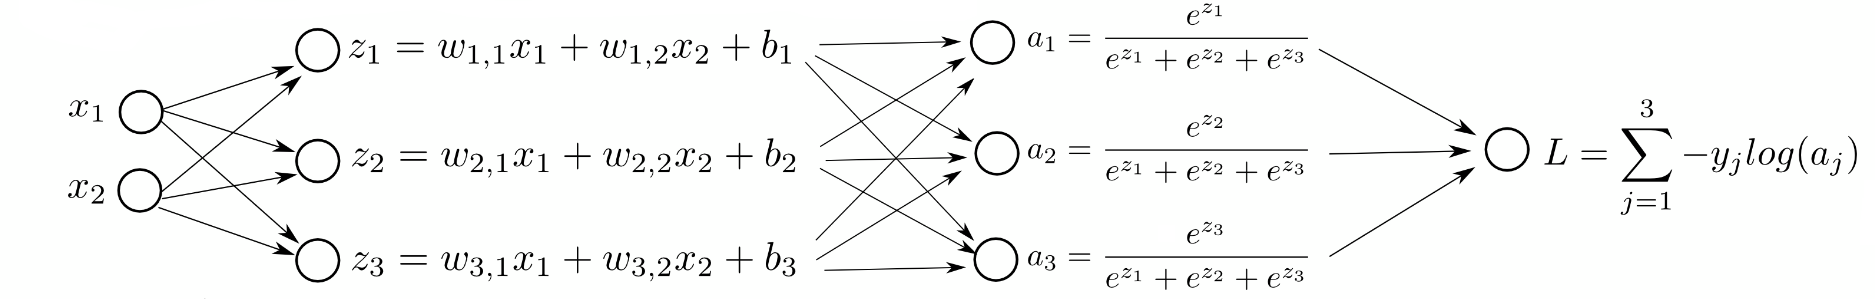
\includegraphics[width=\textwidth]{images/softmax_neural_network.png}
\end{widget}
\caption{Il softmax come rete neurale con due feature e tre classi: dai logit $z_i = w_{i,1}x_1 + w_{i,2}x_2 + b_i$ alle probabilità $a_i = e^{z_i}/\sum_{k=1}^{3}e^{z_k}$, fino alla cross-entropy loss $L = \sum_{j=1}^{3} -y_j\log(a_j)$. Il bias $b_i$ corrisponde al parametro $\vartheta_0^{(i)}$ associato alla feature $x_0 = 1$.}
\label{fig:softmax-nn}
\end{figure}

\paragraph{Esempio.}
Consideriamo tre classi e un input con due feature, $x = [1,\ 0.2,\ 0.1]^T$ (la prima componente è il bias). Siano i parametri, scritti per righe (una riga per classe):
\[
\vartheta^T =
\begin{bmatrix}
-1 & 1 & 0 \\
1 & 0.5 & 1 \\
2 & 1 & 1.5
\end{bmatrix}
\]
e supponiamo che la classe corretta sia la prima, $y = [1, 0, 0]^T$.

\textbf{Soluzione.} Calcoliamo in ordine i tre ingredienti del softmax:
\begin{center}
\begin{tabular}{@{}cccc@{}}
\toprule
Classe & Modello lineare $z_k$ & Logit $e^{z_k}$ & Normalizzazione $p_k$ \\
\midrule
0 & $-1 + 0.2 + 0 = -0.8$ & $0.45$ & $0.03$ \\
1 & $1 + 0.1 + 0.1 = 1.2$ & $3.32$ & $0.23$ \\
2 & $2 + 0.2 + 0.15 = 2.35$ & $10.49$ & $0.74$ \\
\midrule
 & & $\sum = 14.26$ & $\sum = 1$ \\
\bottomrule
\end{tabular}
\end{center}
Il modello assegna alla classe corretta una probabilità di appena $0.03$, per cui la loss su questo campione è alta: $L = -1\cdot\log(0.0315) \approx 3.46$. La loss complessiva si ottiene facendo la media di questi valori su tutti gli $m$ campioni del training set.

\begin{figure}[htbp]
\centering
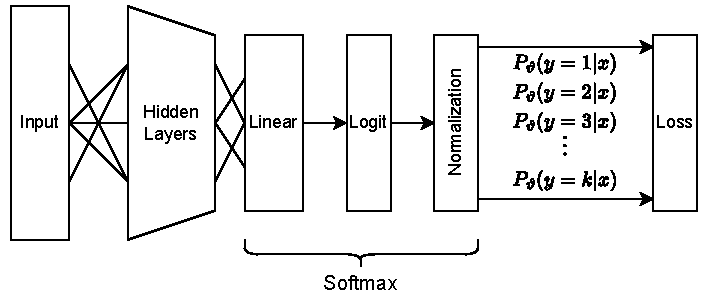
\includegraphics[width=0.85\textwidth]{images/neural-net.pdf}
\caption{Struttura ``standard'' di una rete neurale per la classificazione: dopo l'input e gli hidden layer, gli ultimi blocchi (modello lineare, logit e normalizzazione) sono esattamente un softmax, che produce le probabilità $P_\vartheta(y = k \mid x)$ su cui viene calcolata la loss.}
\label{fig:nn-standard}
\end{figure}

\section{Loss function e Multi-Class SVM}
Ci si potrebbe chiedere se anche una SVM sia una rete neurale. Una SVM lineare, come il softmax, è una \textbf{macchina lineare}: calcola un vettore di punteggi $f = Wx + b$, uno per classe. Ciò che cambia tra i due modelli è soltanto la funzione di loss: cambiando la loss di questo framework lineare si ottiene la \textbf{Multi-Class SVM}, che usa la \textbf{hinge loss}:
\[
L = \underbrace{\frac{1}{N}\sum_{i}\sum_{j \neq y_i}\max(0,\ f_j - f_{y_i} + 1)}_{\text{data loss}} + \underbrace{\lambda\sum_{k}\sum_{l}W_{k,l}^2}_{\text{regularization loss}}
\]
dove $f_{y_i}$ è il punteggio della classe corretta. In questo senso una SVM lineare può essere vista come la stessa rete a un solo layer del softmax, con una loss diversa; tipicamente, però, il termine ``rete neurale'' si riserva a modelli che apprendono anche una rappresentazione degli input, come vedremo tra poco.

\paragraph{Esempio.}
Siano $f = [-2.85,\ 0.86,\ 0.28]^T$ i punteggi prodotti da $Wx + b$ per un esempio la cui classe corretta è $y_i = 2$, ovvero quella con punteggio $0.28$.

\textbf{Soluzione.} Con la hinge loss si sommano i contributi delle classi errate:
\[
L_{\text{hinge}} = \max(0,\ -2.85 - 0.28 + 1) + \max(0,\ 0.86 - 0.28 + 1) = 0 + 1.58 = 1.58.
\]
Con la cross-entropy, invece, si applicano esponenziale e normalizzazione,
\[
e^{f} = [0.058,\ 2.36,\ 1.32]^T \quad\Longrightarrow\quad p = [0.015,\ 0.631,\ 0.353]^T,
\]
e si prende il logaritmo della probabilità della classe corretta: $L_{\text{CE}} = -\log(0.353) \approx 1.04$.

\paragraph{Loss per la classificazione binaria.}
In generale, la loss complessiva è la somma delle loss sui singoli esempi, $L = \sum_{i=1}^{m}\mathrm{loss}\big(f(x^{(i)}), y^{(i)}\big)$. Nel caso binario, con $y^{(i)} \in \{-1, +1\}$, alcuni esempi sono:
\begin{itemize}
    \item \textbf{Zero-one loss}: $\mathbf{1}\{\mathrm{sign}(f(x^{(i)})) \neq y^{(i)}\}$, che conta gli errori ma non è né continua né derivabile.
    \item \textbf{Hinge loss}: $\max\big(0,\ 1 - f(x^{(i)})\,y^{(i)}\big)$, usata dalle SVM.
    \item \textbf{Logistic loss}: $\log\big(1 + \exp(-f(x^{(i)})\,y^{(i)})\big)$, usata dalla regressione logistica.
\end{itemize}
Allo stesso modo, la regressione lineare usa la \textbf{least squares loss} $\frac{1}{2}(y - z)^2$, mentre le reti neurali per la classificazione usano la cross-entropy. In tutti i casi la funzione di costo da minimizzare con la discesa del gradiente è $J(\vartheta) = \sum_{i=1}^{m} L\big(h_\vartheta(x^{(i)}), y^{(i)}\big)$, e il modello restituisce un valore continuo nella regressione o una classe nella classificazione.

\section{Il ruolo della rappresentazione}
Un modello lineare come il softmax produce sempre decision boundary lineari: funziona bene quando i dati sono \textbf{linearmente separabili}, ma fallisce quando non lo sono, come nel caso di due classi disposte a cerchi concentrici. Una soluzione nota è quella di trasformare le feature con una funzione $\phi(x)$, ad esempio un kernel, che mappa i dati in uno spazio a dimensione più alta in cui diventano separabili da un iperpiano (figura~\ref{fig:kernel}).

\begin{figure}[htbp]
\centering
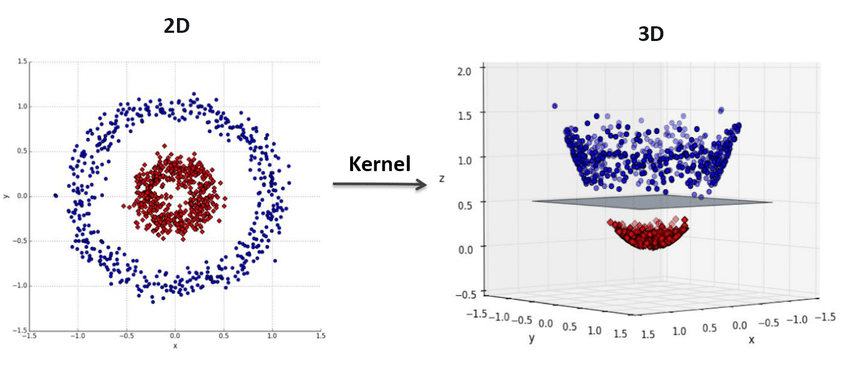
\includegraphics[width=0.75\textwidth]{images/non_linear_SVM.png}
\caption{Dati non linearmente separabili nello spazio di input bidimensionale (a sinistra): due classi disposte a cerchi concentrici. Applicando una trasformazione $\phi$ che aggiunge una dimensione (a destra), le due classi diventano separabili da un piano nello spazio delle feature.}
\label{fig:kernel}
\end{figure}

Il problema è che scegliere la $\phi(x)$ giusta non è semplice: dipende dai dati e dal task, e una rappresentazione costruita a mano (\emph{hand crafted}) potrebbe non essere quella migliore. La domanda diventa allora: possiamo \textbf{apprendere} la funzione $\phi(x)$ direttamente dai dati? La risposta sono le reti neurali e il Deep Learning, che fanno \textbf{representation learning}, ovvero imparano in modo supervisionato, a seconda del task, come trasformare l'input in una rappresentazione utile.

\section{Reti neurali}\label{sec:reti-neurali}
La prima rete neurale studiata fu il \textbf{percettrone} di Rosenblatt, ovvero un singolo neurone che calcola una somma pesata degli input (con la soglia incorporata come peso $\vartheta_0$ del bias $x_0 = 1$) e restituisce un'uscita binaria. Il percettrone è dotato di una procedura di learning automatico dei pesi, ma, come tutti i modelli lineari, risolve solo problemi linearmente separabili: non è in grado, ad esempio, di calcolare lo XOR.

\begin{figure}[htbp]
\centering
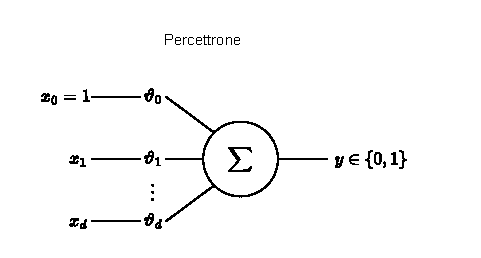
\includegraphics[width=0.5\textwidth]{images/percettrone.pdf}
\caption{Il percettrone di Rosenblatt: le feature $x_1, \dots, x_d$ e il bias $x_0 = 1$ vengono pesati dai parametri $\vartheta_0, \dots, \vartheta_d$ e sommati; l'uscita è binaria, $y \in \{0, 1\}$.}
\label{fig:percettrone}
\end{figure}

\subsection{Multi-Layer Perceptron}
Il \textbf{Multi-Layer Perceptron} (MLP) nasce da due motivazioni:
\begin{enumerate}
    \item Dobbiamo adattare il modello a dati che vivono in uno spazio non lineare, come nel problema dello XOR.
    \item Dato un insieme di dati (ad esempio immagini o documenti di testo), dobbiamo imparare una buona rappresentazione di essi, e non usarne una costruita a mano.
\end{enumerate}

Un MLP è organizzato a strati: un \textbf{input layer}, uno o più \textbf{hidden layer} e un \textbf{output layer}, in cui ogni neurone di un layer è connesso a tutti i neuroni del layer successivo (figura~\ref{fig:mlp}). Ogni layer, ad eccezione dell'output, contiene anche un'unità di bias che vale sempre 1.

\begin{figure}[htbp]
\centering
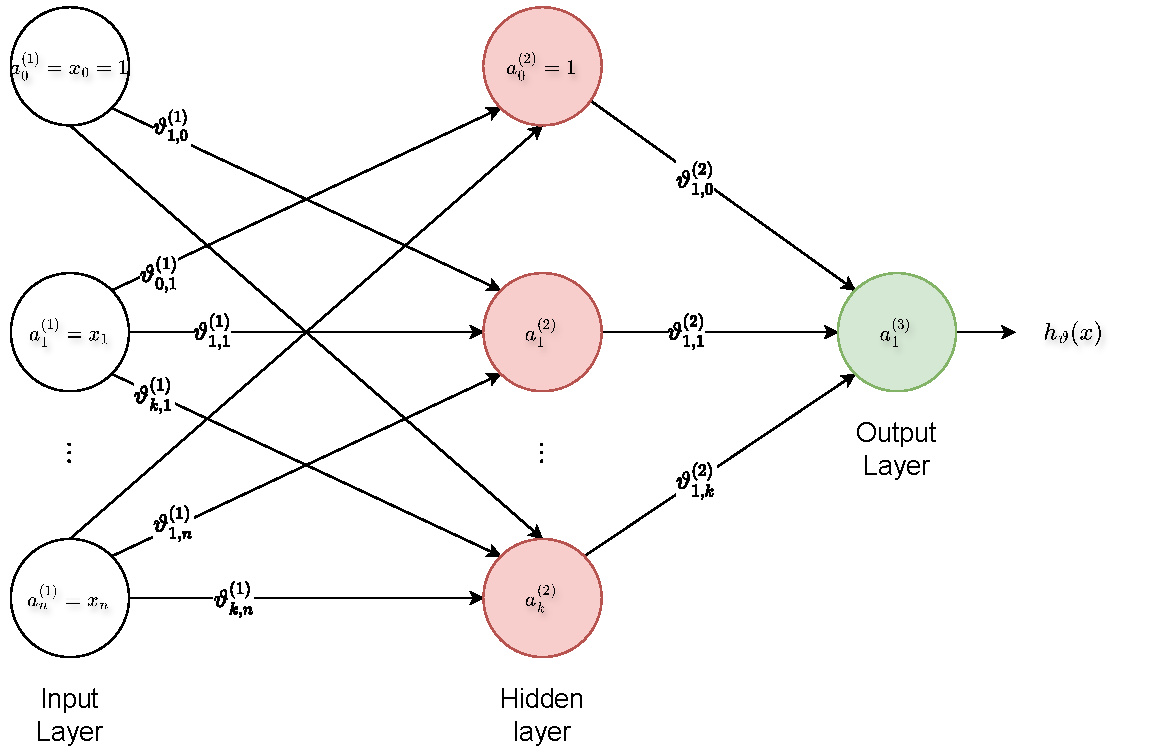
\includegraphics[width=0.75\textwidth]{images/NeuralNet1pdf.pdf}
\caption{Un Multi-Layer Perceptron con un input layer (in bianco, $a_i^{(1)} = x_i$), un hidden layer con $k$ neuroni (in rosso) e un output layer con un solo neurone (in verde) che restituisce $h_\vartheta(x)$. Le unità $a_0^{(1)}$ e $a_0^{(2)}$ sono i bias, sempre pari a 1; i pesi $\vartheta_{ji}^{(l)}$ sono riportati sugli archi.}
\label{fig:mlp}
\end{figure}

\paragraph{Notazione.}
Indichiamo con:
\begin{itemize}
    \item $a_i^{(l)}$ l'\textbf{attivazione} della $i$-esima unità del layer $l$; nell'input layer $a_i^{(1)} = x_i$.
    \item $\vartheta_{ji}^{(l)}$ il parametro che collega l'unità $i$ del layer $l$ (di partenza) all'unità $j$ del layer $l+1$ (di arrivo).
    \item $\vartheta^{(l)}$ la matrice dei parametri che mappa il layer $l$ nel layer $l+1$.
\end{itemize}

Ogni neurone calcola una combinazione lineare delle attivazioni del layer precedente e vi applica una \textbf{funzione di attivazione} $f$:
\[
z_j^{(l)} = \sum_{i} \vartheta_{ji}^{(l-1)}\, a_i^{(l-1)} = \vartheta_{j0}^{(l-1)}a_0^{(l-1)} + \vartheta_{j1}^{(l-1)}a_1^{(l-1)} + \dots, \qquad a_j^{(l)} = f\big(z_j^{(l)}\big)
\]
o, in forma matriciale, $z^{(l)} = \vartheta^{(l-1)}a^{(l-1)}$ e $a^{(l)} = f(z^{(l)})$, dove $f$ è applicata elemento per elemento. Nel caso della figura~\ref{fig:mlp}, l'output della rete è quindi:
\[
\begin{aligned}
h_\vartheta(x) = a_1^{(3)} &= f\big(\vartheta_{10}^{(2)} + \vartheta_{11}^{(2)}a_1^{(2)} + \dots + \vartheta_{1k}^{(2)}a_k^{(2)}\big) \\
&= f\Big(\vartheta_{10}^{(2)} + \vartheta_{11}^{(2)}\underbrace{f\big(\vartheta_{10}^{(1)} + \dots + \vartheta_{1n}^{(1)}a_n^{(1)}\big)}_{a_1^{(2)}} + \dots + \vartheta_{1k}^{(2)}\underbrace{f\big(\vartheta_{k0}^{(1)} + \dots + \vartheta_{kn}^{(1)}a_n^{(1)}\big)}_{a_k^{(2)}}\Big)
\end{aligned}
\]
Una rete neurale è quindi una \textbf{composizione di funzioni derivabili}.

\paragraph{Numero di parametri.}
Se la rete ha $s_l$ unità nel layer $l$ e $s_{l+1}$ unità nel layer $l+1$, la matrice $\vartheta^{(l)}$ ha dimensione $s_{l+1} \times (s_l + 1)$, dove il $+1$ tiene conto dell'unità di bias. Ad esempio, una rete con 2 feature in input, un hidden layer con 3 neuroni e un output layer con 2 neuroni ha $\vartheta^{(1)} \in \mathbb{R}^{3 \times 3}$ e $\vartheta^{(2)} \in \mathbb{R}^{2 \times 4}$, per un totale di $9 + 8 = 17$ parametri.

\subsection{Le due parti di una rete neurale}
Una rete neurale per la classificazione è composta da due parti (figura~\ref{fig:nn-parti}):
\begin{itemize}
    \item \textbf{Feature learning}: la prima parte della rete impara, in modo supervisionato e a seconda del task, come trasformare l'input $x$ in una rappresentazione utile, nell'esempio $a^{(2)}$.
    \item \textbf{Classificatore}: l'ultima parte è un softmax (o una regressione logistica, nel caso binario) che prende in input le feature apprese.
\end{itemize}

\begin{figure}[htbp]
\centering
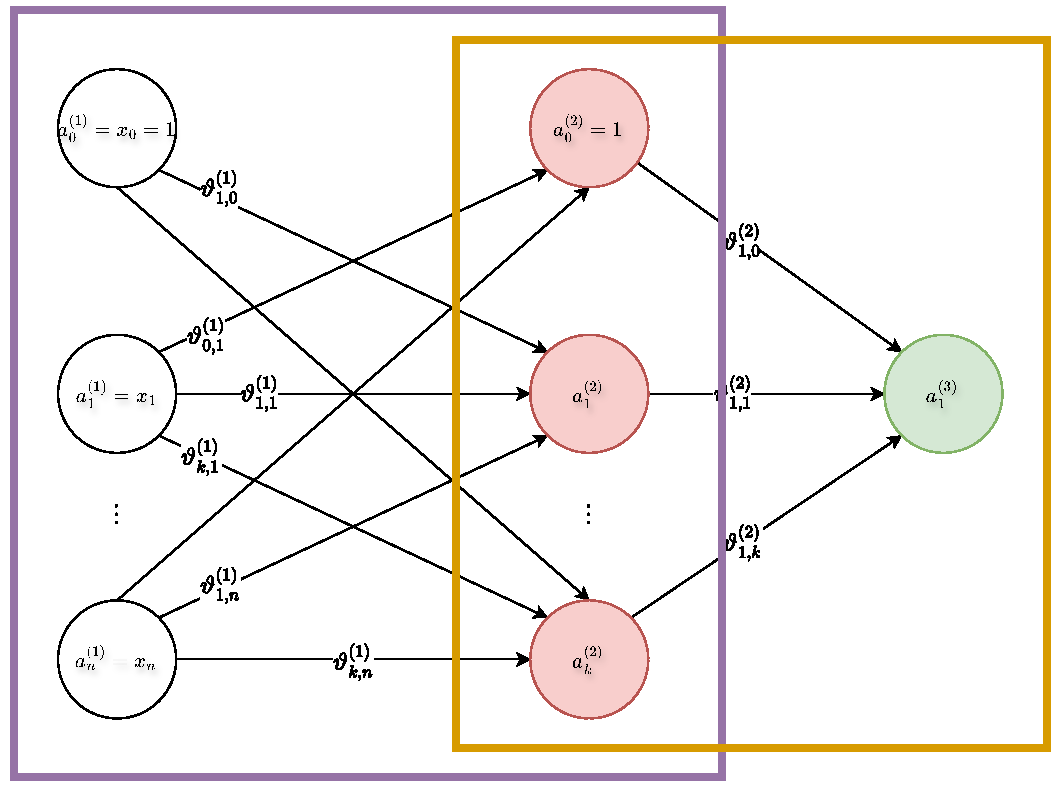
\includegraphics[width=0.7\textwidth]{images/NeuralNet2pdf.pdf}
\caption{Le due parti di una rete neurale: il riquadro viola evidenzia la trasformazione appresa dell'input $x$ nelle feature $a^{(2)}$, mentre il riquadro arancione evidenzia il classificatore (softmax o regressione logistica) che usa le feature apprese.}
\label{fig:nn-parti}
\end{figure}

Si possono aggiungere tutti gli hidden layer necessari per adattare la rete a un problema non lineare, rendendola \textbf{profonda} (\emph{deep}). Hidden layer diversi possono avere un numero diverso di neuroni. La funzione di attivazione, invece, è in genere la stessa per tutti i neuroni (si possono usare funzioni diverse, ma si tratta di casi particolari). Al crescere della dimensione dell'input aumenta la probabilità che lo spazio sia non lineare, e può quindi servire aggiungere layer, neuroni per layer, o entrambi.

\subsection{Funzioni di attivazione}
Le funzioni di attivazione \textbf{devono essere derivabili}: in questo modo la rete, essendo una composizione di funzioni derivabili, è a sua volta derivabile, e la si può addestrare con la discesa del gradiente. Le più usate sono:
\begin{center}
\renewcommand{\arraystretch}{1.6}
\begin{tabular}{@{}lll@{}}
\toprule
Nome & Funzione & Derivata \\
\midrule
Identità & $f(x) = x$ & $f'(x) = 1$ \\
Sigmoide (logistica) & $f(x) = \dfrac{1}{1 + e^{-x}}$ & $f'(x) = f(x)\big(1 - f(x)\big)$ \\
Tangente iperbolica & $f(x) = \tanh(x) = \dfrac{2}{1 + e^{-2x}} - 1$ & $f'(x) = 1 - f(x)^2$ \\
ReLU & $f(x) = \max(0, x)$ & $f'(x) = \mathbf{1}\{x \ge 0\}$ \\
Softplus & $f(x) = \log(1 + e^{x})$ & $f'(x) = \dfrac{1}{1 + e^{-x}}$ \\
\bottomrule
\end{tabular}
\end{center}

\begin{figure}[htbp]
\centering
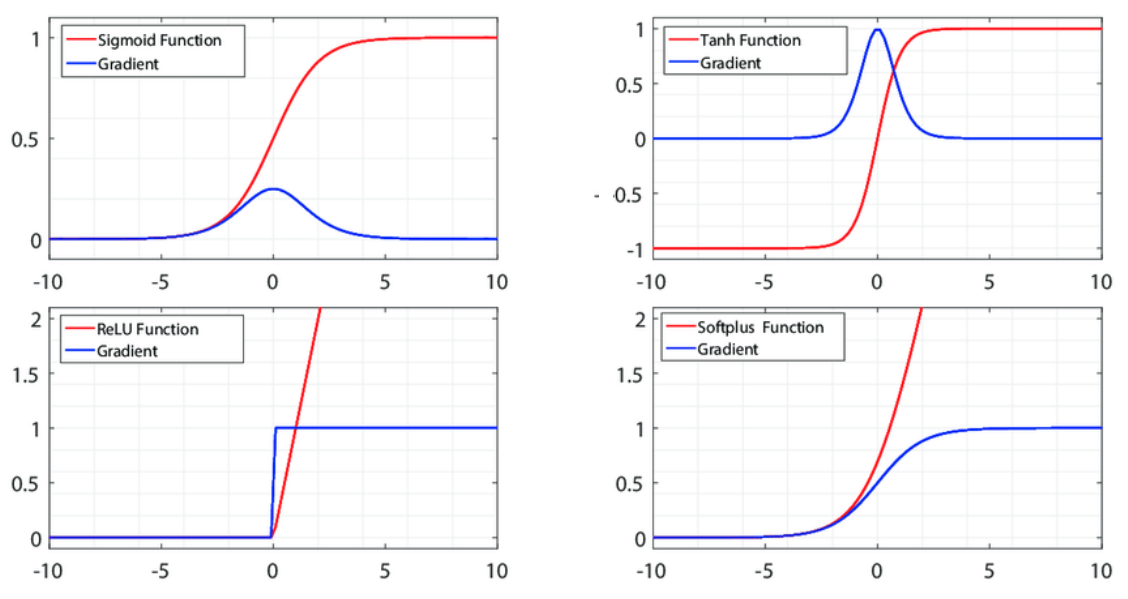
\includegraphics[width=0.8\textwidth]{images/activation-functions.png}
\caption{Le funzioni di attivazione più usate (in rosso) e le relative derivate (in blu): sigmoide (in alto a sinistra), tangente iperbolica (in alto a destra), ReLU (in basso a sinistra) e softplus (in basso a destra). Si noti come la derivata della softplus sia proprio la sigmoide.}
\label{fig:attivazioni}
\end{figure}

\subsection{Il teorema di approssimazione universale}
Il motivo per cui le reti neurali funzionano così bene su problemi non lineari è formalizzato dal seguente risultato.

\begin{teorema}[Approssimazione universale]\label{teo:uat}
Una rete neurale feedforward\footnote{Per feedforward si intende una rete in cui ogni layer riceve input esclusivamente dal layer precedente e lo trasmette al successivo, senza cicli.} con un solo hidden layer, dotata di un numero finito ma sufficientemente grande di neuroni e di una funzione di attivazione non lineare e non polinomiale (ad esempio la sigmoide), è in grado di approssimare qualunque funzione continua $f : C \to \mathbb{R}$ definita su un insieme compatto $C \subset \mathbb{R}^n$ con errore arbitrariamente piccolo, ovvero per ogni $\varepsilon > 0$ esiste una rete che implementa $\hat{f}$ tale che
\[
\sup_{x \in C}\big|f(x) - \hat{f}(x)\big| < \varepsilon.
\]
\end{teorema}

Il teorema garantisce quindi che un solo hidden layer è sufficiente a \emph{rappresentare} qualunque funzione continua, ma non dice nulla su quanto questo sia praticabile: come osservato in \cite{Goodfellow-et-al-2016}, il layer potrebbe dover essere enormemente grande e la rete potrebbe non riuscire ad apprendere e generalizzare correttamente. Il teorema non fornisce infatti né un metodo per trovare i parametri, né un limite al numero di neuroni necessari. In pratica, l'uso di più hidden layer permette spesso di rappresentare le stesse funzioni in modo più compatto: questa è una delle motivazioni delle reti \emph{deep}.

\subsection{Classificazione multiclasse e regressione}
Le reti neurali permettono di addestrare ipotesi complesse e non lineari sullo spazio delle feature, a seconda del task:
\begin{itemize}
    \item \textbf{Classificazione binaria}: basta un solo neurone di output, con $y^{(i)} \in \{0, 1\}$.
    \item \textbf{Classificazione multiclasse}: con $K \ge 3$ classi si usano $K$ unità di output e le etichette sono vettori one-hot, $y^{(i)} \in \{0, 1\}^K$, con un solo 1 nella posizione corrispondente alla classe. Come visto in figura~\ref{fig:nn-standard}, l'output layer è un softmax.
    \item \textbf{Regressione}: si eliminano logit e normalizzazione, si usa una regressione lineare nell'ultimo layer (ogni nodo di output è un regressore lineare) e si cambia la funzione di costo, usando la \textbf{MSE loss}, che deve tenere conto dell'output di tutti i regressori (figura~\ref{fig:nn-regressione}).
\end{itemize}

\begin{figure}[htbp]
\centering
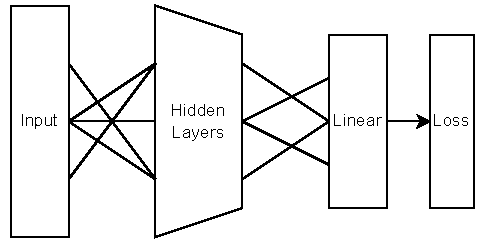
\includegraphics[width=0.6\textwidth]{images/linear-reg-neuralnet.pdf}
\caption{Struttura di una rete neurale per la regressione: dopo gli hidden layer l'ultimo blocco è un modello lineare, la cui uscita viene confrontata con il target tramite la MSE loss.}
\label{fig:nn-regressione}
\end{figure}

\section{Training e inferenza}
Supponiamo di aver definito un'architettura. Durante la fase di \textbf{training} l'obiettivo è imparare i parametri migliori per il modello, e per farlo servono una funzione di loss e un algoritmo che li apprenda. Una volta ottenuti i parametri, questi vengono usati per fare \textbf{inferenza} su nuovi pattern.

\paragraph{Funzione di costo.}
Per la classificazione vogliamo trovare $\hat{\vartheta}$ tale che
\[
\hat{\vartheta} = \arg\min_\vartheta J(\vartheta), \qquad J(\vartheta) = -\frac{1}{m}\sum_{i=1}^{m}\sum_{c=0}^{K-1}\mathbf{1}\{y^{(i)} = c\}\log h_\vartheta^{(c)}(x^{(i)})
\]
ovvero la somma delle cross-entropy di tutti i neuroni di output. Per raggiungere l'obiettivo dobbiamo essere in grado di calcolare in modo efficiente
\[
\frac{\partial J(\vartheta)}{\partial \vartheta_{ji}^{(l)}} \qquad \forall j, i, l.
\]

\paragraph{Overfitting.}
Le dimensioni della rete determinano un trade-off. Una rete ``piccola'' ha pochi parametri, è computazionalmente più economica ma è più soggetta a underfitting. Una rete ``grande'' ha molti parametri, è più soggetta a overfitting ed è computazionalmente più costosa; in questo caso si usa la regolarizzazione ($\lambda$) per contrastare l'overfitting.

\paragraph{Inizializzazione dei parametri.}
Come inizializzare la matrice dei parametri $\vartheta$? Se si assegnassero gli stessi valori ai pesi che partono dallo stesso nodo, i nodi di arrivo calcolerebbero esattamente le stesse cose e riceverebbero gli stessi gradienti, comportandosi come un unico neurone. Per questo motivo si effettua il \textbf{symmetry breaking}: i parametri che dipendono dallo stesso nodo devono essere inizializzati con valori diversi e piccoli, tipicamente scelti casualmente in un intervallo $\vartheta_{ji}^{(l)} \in [-\varepsilon, \varepsilon]$.

\section{Come si apprendono i parametri?}\label{sec:problema-learning}
Arriviamo così al problema centrale: come si apprendono i parametri di una rete neurale con un numero di hidden layer $\geq 1$? Riepilogando quanto visto finora:
\begin{itemize}
    \item \textbf{Un solo neurone}: si usa la discesa del gradiente, evoluzione dell'algoritmo di learning di Rosenblatt.
    \item \textbf{Softmax}: si usa la discesa del gradiente, perché la loss agisce su un solo layer di pesi.
    \item \textbf{Rete con hidden layer}: i valori dei nodi nascosti non sono noti in anticipo, ovvero il training set non fornisce alcuna ground truth per i layer intermedi.
\end{itemize}
Di conseguenza non possiamo più usare la discesa del gradiente nella forma classica, ma dobbiamo rivedere il modo in cui calcoliamo le derivate rispetto ai parametri. La soluzione si basa sul fatto che le reti neurali sono \textbf{grafi computazionali}, su cui si può usare la \textbf{chain rule} per spostare i gradienti all'indietro: è l'algoritmo di \textbf{backpropagation}, oggetto del prossimo capitolo.

In sintesi, il softmax risolve la classificazione multiclasse ma resta un modello lineare; le reti neurali imparano anche la rappresentazione dei dati e possono approssimare funzioni non lineari arbitrarie, al prezzo di dover calcolare i gradienti rispetto a parametri di layer di cui non conosciamo l'uscita attesa.

\section*{Riferimenti}
Il materiale visto in questo capitolo comprende:
\begin{itemize}
    \item Materiale visto a lezione (13 ottobre 2026).
    \item Slide del corso \emph{Softmax -- Generalization of Logistic Regression} e \emph{Neural Network -- Multi-Layer Perceptron \& Deep Learning}.
    \item Riassunto dei capitoli 2, 4 e 6 delle dispense di \emph{Machine Learning}, da cui sono tratte anche tutte le figure di questo capitolo: \url{https://github.com/emanuelegaliano/Machine-Learning}.
    \item Teorema di approssimazione universale dal libro \citetitle{Goodfellow-et-al-2016} \cite{Goodfellow-et-al-2016}, sezione 6.4.1.
\end{itemize}
